% !TEX program = lualatex
\documentclass[12pt,a4paper]{article}
\usepackage{fontspec}
\setmonofont{Latin Modern Mono}
\usepackage{xcolor}
\usepackage{listings}
\usepackage{geometry}
\usepackage{fancyhdr}
\usepackage{hyperref}
\usepackage{graphicx}
\geometry{margin=0.3in}
\usepackage{multicol}

% ===============================
% Toggle to show / hide solutions
% ===============================
\newif\ifshowsolutions
\showsolutionstrue
% \showsolutionsfalse

% -------------------------------
% Header and Footer Configuration
% -------------------------------
\pagestyle{fancy}
\fancyhf{}
\lhead{Lab Mid}
\rhead{CSE 4308: DBMS Lab}
\cfoot{\thepage}
\setlength{\headwidth}{\textwidth}

% -------------------------------
% Code Listing Style
% -------------------------------
\definecolor{codegreen}{rgb}{0,0.6,0}
\definecolor{codegray}{rgb}{0.5,0.5,0.5}
\definecolor{codepurple}{rgb}{0.58,0,0.82}
\definecolor{backcolour}{rgb}{0.95,0.95,0.92}

\lstdefinestyle{mystyle}{
    backgroundcolor=\color{backcolour},
    commentstyle=\color{codegreen},
    keywordstyle=\color{magenta},
    numberstyle=\tiny\color{codegray},
    stringstyle=\color{codepurple},
    basicstyle=\ttfamily\footnotesize,
    breaklines=true,
    captionpos=b,
    keepspaces=true,
    numbers = none,
    numbersep=5pt,
    tabsize=2,
    frame=single,
    columns=fullflexible,
    showspaces=false,
    showstringspaces=false,
    showtabs=false
}

\lstset{style=mystyle}

% Images: found next to this file (local compile_labs.sh) or via the
% lab folder when compiled from the project root (Overleaf).
\graphicspath{{lab_08_mid/}}

\begin{document}

% --------------------------------------------------------------
% TITLE PAGE
% --------------------------------------------------------------
\begin{titlepage}
\centering
\vspace*{2\baselineskip}

\rule{14cm}{2pt}\vspace*{-0.8\baselineskip}\vspace*{1.5pt}
\rule{14cm}{0.5pt}\vspace{2\baselineskip}

{\Huge\bfseries\scshape Lab Mid\par}

\rule{14cm}{0.5pt}\vspace*{-0.7\baselineskip}\vspace{2.5pt}
\rule{14cm}{2pt}

\vspace{2\baselineskip}

{\Large\bfseries CSE 4308\par}
{\large DATABASE MANAGEMENT SYSTEMS LAB\par}

\vfill
{\normalsize Prepared by:\\ Samnun Azfar, Jr. Lecturer, CSE\\ Samia Nawsheen, Jr. Lecturer, CSE\par}
{\normalsize Academic Year: AY25-26\par}
\end{titlepage}

\newpage

\section*{DBMS Lab Mid}

\begin{figure}[h]
% \centering
\hspace{-1.5cm}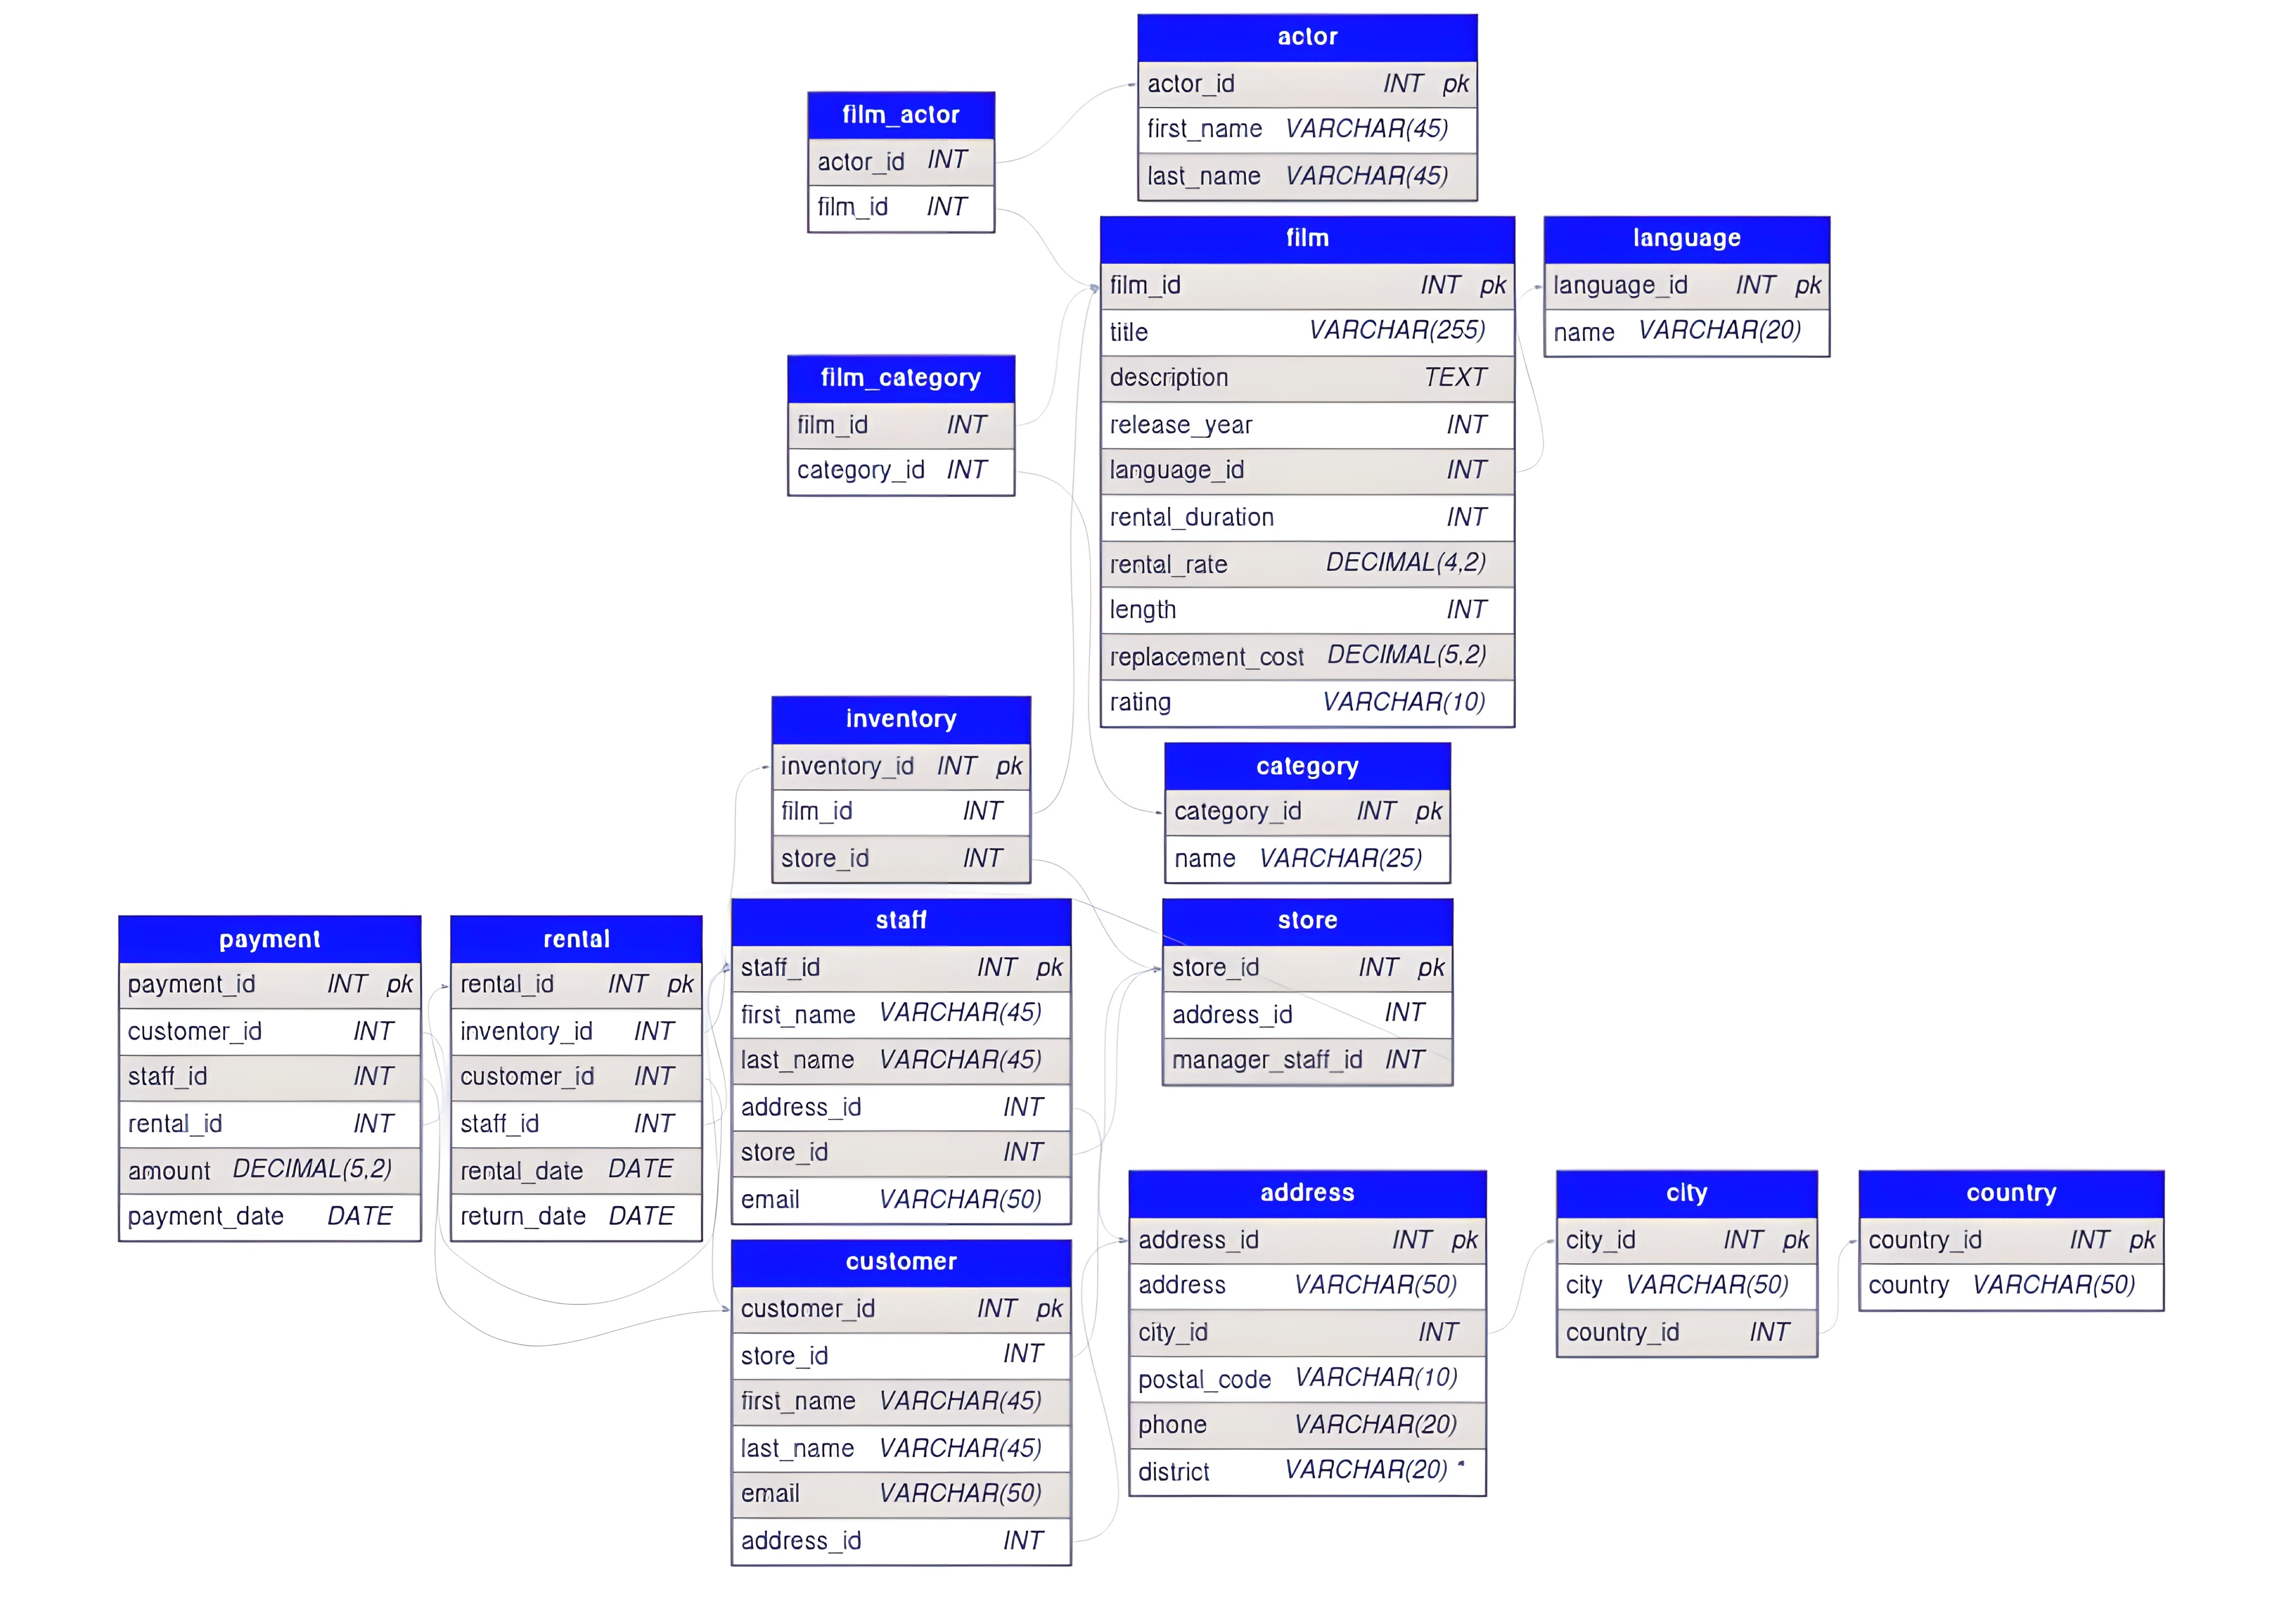
\includegraphics[width=22.5cm]{lab_08_dvdrental_1.png}
\end{figure}

\begin{enumerate}

% --------------------------------------------------

\item Find distinct customers who have made payments of amount 0.

\ifshowsolutions
\textbf{Solution:}
\begin{lstlisting}[language=SQL]
SELECT DISTINCT c.customer_id, c.first_name, c.last_name, c.email, p.amount
FROM customer c
JOIN payment p ON c.customer_id = p.customer_id
WHERE p.amount = 0;
\end{lstlisting}
\fi

% --------------------------------------------------

\item Display only the username part of staff emails (everything before @).

\ifshowsolutions
\textbf{Solution:}
\begin{lstlisting}[language=SQL]
SELECT SUBSTR(email, 1, POSITION('@' IN email) - 1) AS username
FROM staff;
\end{lstlisting}
\fi

% --------------------------------------------------

\item For each customer, count the total number of rentals they have made, sorted in descending order.

\ifshowsolutions
\textbf{Solution:}
\begin{lstlisting}[language=SQL]
SELECT c.first_name, c.last_name, COUNT(r.rental_id) AS total_rentals
FROM customer c
LEFT JOIN rental r ON c.customer_id = r.customer_id
GROUP BY c.customer_id
ORDER BY total_rentals DESC;
\end{lstlisting}
\fi

% --------------------------------------------------

\item List the first name and last name of staff members along with the total amount collected by each in payments.

\ifshowsolutions
\textbf{Solution:}
\begin{lstlisting}[language=SQL]
SELECT s.first_name, s.last_name, SUM(p.amount) AS total_collected
FROM staff s
LEFT JOIN payment p ON s.staff_id = p.staff_id
GROUP BY s.staff_id;
\end{lstlisting}
\fi

% --------------------------------------------------

\item Identify the top 5 customers who spent the highest total payment amount.

\ifshowsolutions
\textbf{Solution:}
\begin{lstlisting}[language=SQL]
SELECT c.first_name, c.last_name, SUM(p.amount) AS total_paid
FROM customer c
JOIN payment p ON c.customer_id = p.customer_id
GROUP BY c.customer_id
ORDER BY total_paid DESC
LIMIT 5;
\end{lstlisting}
\fi

% --------------------------------------------------

\item List rentals that were returned more than 7 days after the rental date.
Show rental\_id, rental\_date, return\_date, and total number of days rented.

\ifshowsolutions
\textbf{Solution:}
\begin{lstlisting}[language=SQL]
SELECT rental_id, rental_date, return_date, return_date - rental_date AS days_rented
FROM rental
WHERE return_date - rental_date > INTERVAL '7 days';
\end{lstlisting}
\fi

% --------------------------------------------------

\item For each staff member, show their full name and the latest rental date they handled.

\ifshowsolutions
\textbf{Solution:}
\begin{lstlisting}[language=SQL]
SELECT s.first_name || ' ' || s.last_name AS staff_name, MAX(r.rental_date) AS latest_rental
FROM staff s
JOIN rental r ON s.staff_id = r.staff_id
GROUP BY s.staff_id;
\end{lstlisting}
\fi

% --------------------------------------------------

\item Display the title, rating, and rental rate of all films whose rental rate is greater than 4.00 and whose rating is either ``PG" or ``PG-13".

\ifshowsolutions
\textbf{Solution:}
\begin{lstlisting}[language=SQL]
SELECT title, rating, rental_rate
FROM film
WHERE rental_rate > 4.00 AND rating IN ('PG', 'PG-13');
\end{lstlisting}
\fi

% --------------------------------------------------

\item Find all customers who live in a city that belongs to the country \texttt{India}, showing the customer's first and last name, city and country.

\ifshowsolutions
\textbf{Solution:}
\begin{lstlisting}[language=SQL]
SELECT 
    c.first_name, 
    c.last_name, 
    c.email, 
    ci.city, 
    co.country
FROM customer c
JOIN address a ON c.address_id = a.address_id
JOIN city ci ON a.city_id = ci.city_id
JOIN country co ON ci.country_id = co.country_id
WHERE co.country = 'India';
\end{lstlisting}
\fi

% --------------------------------------------------

\item List the titles of films in the \texttt{Comedy} category that have a \texttt{length} greater than the average duration of all \texttt{Comedy} films.

\ifshowsolutions
\textbf{Solution:}
\begin{lstlisting}[language=SQL]
SELECT f.title, f.length
FROM film f
JOIN film_category fc ON f.film_id = fc.film_id
JOIN category c ON fc.category_id = c.category_id
WHERE c.name = 'Comedy'
AND f.length > (
    -- Subquery: Calculate average length of Comedy films
    SELECT AVG(f2.length)
    FROM film f2
    JOIN film_category fc2 ON f2.film_id = fc2.film_id
    JOIN category c2 ON fc2.category_id = c2.category_id
    WHERE c2.name = 'Comedy'
);
\end{lstlisting}
\fi

\end{enumerate}

\end{document}
